
\subsection{Overview}

\sidebyside{0.4}{
  A general flow would proceed as follows:

  \begin{enumerate}
    \item Pre-commit picture building
    \item Commit (NLT 45nm)
    \item Target
    \item Meld/Sort (NLT 40nm)
    \item Shoot-Crank (NLT 35nm)
    \item Decide (NLT MAR)
    \item Skate/Banzai
  \end{enumerate}%

}{%
  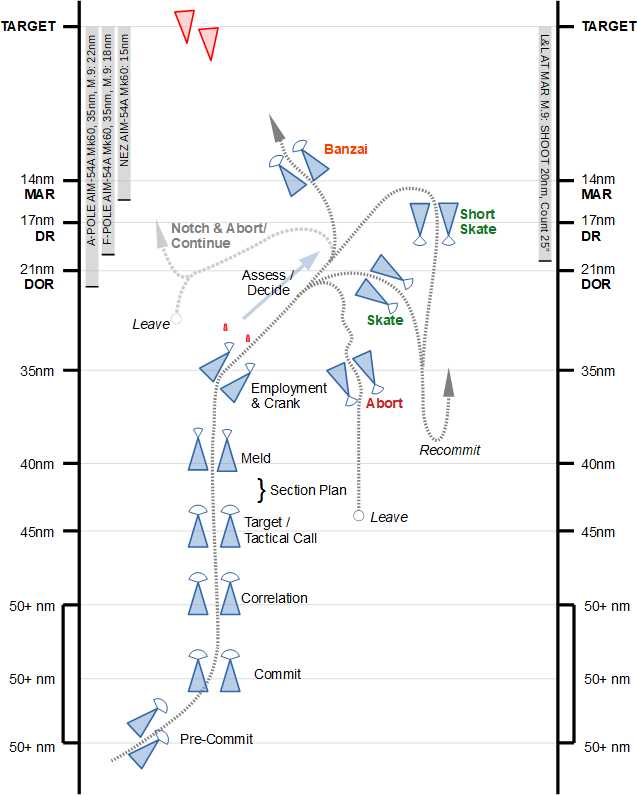
\includegraphics[width=\textwidth,align=t]
    {bvr/bvr-3-timeline-flow-complete-new-1}%
}


The Timeline is a linear process, bound in time segments, to ensure actions
are completed at a perfectly timed point. This is to ensure actions performed
at speed and under stress are completed as a drill.

\begin{enumerate}

  \item At first the friendly fighter group is listening to pictures from AIC
    until they decide to commit to the picture.

  \item The commitment must be prior to passing 45nm distance to the group for
    a valid time line in the Tomcat to be completed advantageously.

  \item At this point they call out that they are targeting the group of
    interest so everyone knows.

  \item At 40nm the flight Lead RIO will call out for MELD on the GROUP and the
    flight will tune their radars and sort on their particular bandit for the
    shot.

  \item At 35nm the Flight will shoot and crank as a section.

  \item Upon Missile Active or Timeout, but NLT Minimum Abort Range, they will
    notch and assess and decide if going Banzai or Skate.

\end{enumerate}
